We have derived MFT predictions about the SPM, and have indications about when those predictions might become invalid, which we tested numerically.
We chose to calculate using the \texttt{KMCLib}\cite{leetmaa2014kmclib} package, which implements the Kinetic Monte Carlo algorithm
(essentially the same as the Gillespie algorithm\cite{Gillespie1977})
on lattice systems. The codes used are kept here~\cite{jHellGitRepo}.
%\texttt{KMCLib} has the advantage that it is python-wrapped \texttt{C++}, and thus quite easy to use whilst at the same time being quite computationally efficient; thus it was fairly easy for us to carry out large numbers
%of differently-parametrised serial \texttt{KMCLib} jobs on the \texttt{Eddie3} computing cluster here at Edinburgh. 
As we have MFT predictions about flow in a block, we can simulate that situation using KMC. In the bulk, the transition rates are simply those described in Fig.~\ref{fig:rates}. At the boundaries
there are 2 layers of lattice sites what switch between being full and empty with rates such that the time-averaged occupation can be specified to match the desired boundary conditions; there are then chances for particles to appear
and disappear with rates depending upon the occupation of these boundary layers. In the end, the intention is that these boundaries should reproduce the effect of having particle reservoirs attached to the edges of the domain,
which is something we check
in the output by inspecting the time-averaged occupations of sites near the boundary. We have used this setup to explore three scenarios, discussed in the following sections. In each of these we refer to a boundary condition configuration
by $(\rho_0, \rho_L)$, with $\rho_0$ and $\rho_L$ being the bottom and top boundary densities respectively.
Measuring overall particle flow rate with such a setup is fairly simple, as we know how many particles enter and leave in a given time.
We can also calculate the time-averaged total number of particles in the system; this is done by updating a histogram of particle numbers
as the simulation progresses. In each of our calculations, we make the initial configuration by randomly filling the system with particles and vacancies in such a way that the initial density should be $\frac{1}{2}(\rho_0 + \rho_L)$, and then
run the system for a sufficient number of equilibration steps to destroy any initial transients.

The MFT suggests that a  transition from a steady flow regime to a critically slow flow regime might occur as the stickiness varies.
We test this by holding the boundary densities constant
whilst changing $\lambda$, and measuring the particle density as well as the mean, variance and skewness of the flow rate. If such a transition does indeed occur, we should expect to see a divergence in one of these moments.
We have done this with four sets of boundary conditions as shown in Fig.~\ref{fig:lambdaScans}. 
\iffalse
\begin{figure*}[h!]
\vspace{1em}
\caption{\label{fig:lambdaScans} Descriptive statistics of flow rates and average overall densities observed when varying $\lambda$ with fixed boundary densities $(\rho_0, \rho_L)$; data series are labelled in the plot.
In the case of the mean flow we have an MFT prediction, indicated by the solid line.
In each case we used systems of length $64$ (length $32$ gives similar results),
running them for $400000$ Gillispie steps for equilibration followed by $10000$ measurement runs of $1000$ steps interspersed with relaxation runs of $16000$
steps. This way we could gather statistics about flow rates and densities in a well-equilibrated system. Specifically, we generate a pool of $10000$ samples of flow rate and density,
from which we can calculate estimates of the descriptive statistics of both quantities.}
\begin{center}
 \begin{tabular}{c|c}
    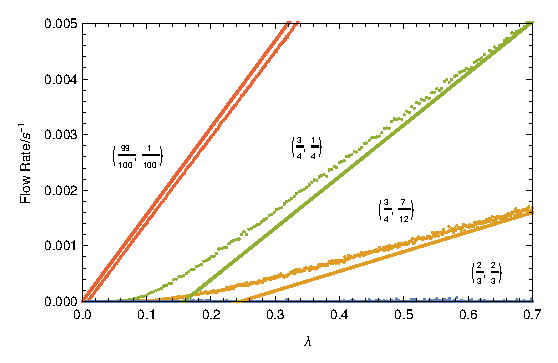
\includegraphics[width=0.5\linewidth]{../tex-src/images/lambdaScan/newFlowMean} & 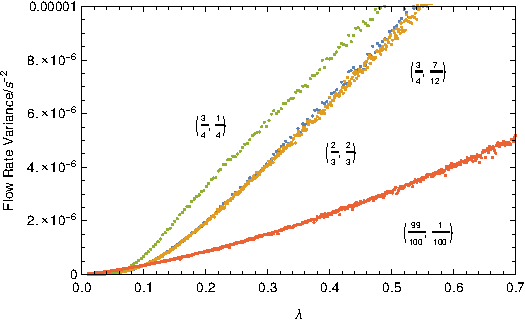
\includegraphics[width=0.5\linewidth]{../tex-src/images/lambdaScan/newFlowVar} \\
    \hline
    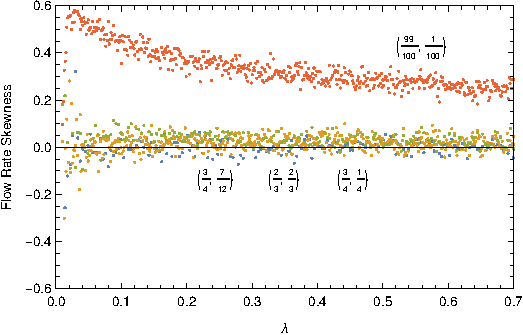
\includegraphics[width=0.5\linewidth]{../tex-src/images/lambdaScan/newFlowSkew} & 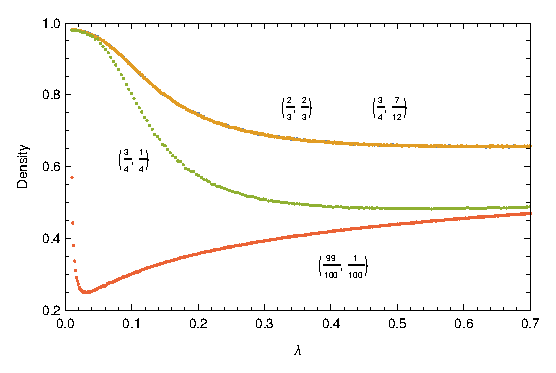
\includegraphics[width=0.5\linewidth]{../tex-src/images/lambdaScan/newDens} \\
    \end{tabular}
\end{center}
    \vspace{-0em}
\end{figure*}
\fi
\begin{figure}[h!]
\vspace{1em}
\caption{\label{fig:lambdaScans} Mean flow rate observed when varying $\lambda$ with fixed boundary densities $(\rho_0, \rho_L)$; data series are labeled in the plot.
The MFT prediction is indicated by the solid line.
In each case we used systems of length $64$ (length $32$ gives similar results),
running them for $400000$ Gillispie steps for equilibration followed by $10000$ measurement runs of $1000$ steps interspersed with relaxation runs of $16000$
steps. This way we could gather statistics about flow rates and densities in a well-equilibrated system. Specifically, we generate a pool of $10000$ samples of flow rate and density
from which we can calculate estimates of the descriptive statistics of both quantities; flow moments and the density data are included in the supplementary materials.
\vspace{1em}}
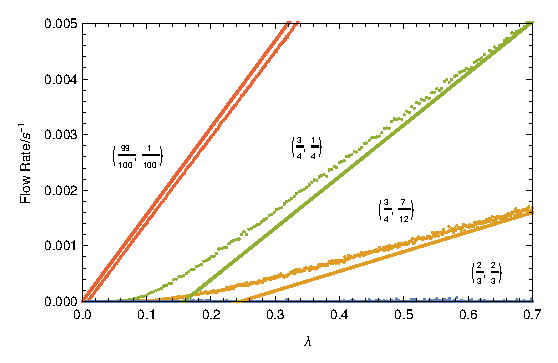
\includegraphics[width=0.98\linewidth]{../tex-src/images/lambdaScan/newFlowMean}
    \vspace{-1em}
\end{figure}

Firstly, we should note that we only have an MFT prediction for the flow rate as a function of $\lambda$, since $\rho(x)$ stops being unique when $\lambda$ drops below $\frac{1}{4}$,
and so the MFT lacks predictive power. For low-stickiness, when $\lambda>\frac{1}{4}$, the MFT is in good agreement with the simulations.
However, one of the key predictions of the MFT - that a sharp transition to a no-flow regime occurs when $\lambda$ becomes small enough (at least for 3 of the 4 sets of
boundary conditions we investigated here) - is not realized in our simulations. Indeed what seems to be happening is that the sharp transition has been smoothed out, as we
do not see any peaks or jumps in the flow rate variance or skewness (which we would expect to see if there was a transition). We suspect that this discrepancy is due to nontrivial correlations emerging between the particles, which the MFT
does not take account of. Alternatively, it could be that the continuum assumption is failing due to the finite-sized system filling with particles and blocking.
\iffalse 
As for the observed average density, for larger $\lambda$ the density approaches the average of the boundary densities,
and for small $\lambda$ the density approaches $1$ (which makes sense as the particles are very strongly attracted to each other, and so the system has a tendency to fill up); the exception to this it the case with extreme full/empty boundary
conditions, although in this case one might argue that the particles are ``sucked out'' of the system so rapidly at the empty end that the system never really has a chance to fill up. It is also worth noticing that this extreme case is the only
one in which the flow rate skewness does anything interesting; it is mostly positive, especially at low-$\lambda$, implying that most of the time the system is fairly static, but occasionally short-lived strong flows occur which end up causing
most of the bulk flow.
\fi

Another situation we can investigate has boundaries $(\rho_B, \rho_T) = (\rho_M + \frac{1}{2} \delta\rho, \rho_M - \frac{1}{2} \delta\rho)$ for some given $\rho_M$, where $\delta\rho$ and $\lambda$ are varied. As before, we calculated flow rate
moments and average densities, and the results are displayed in Fig.~\ref{fig:constDens}. 
\iffalse
\begin{figure*}[h!]
\vspace{1em}
\caption{\label{fig:constDens} Flow rate mean, flow variance and average overall densities observed when varying the difference $\delta\rho$ between the boundary concentrations
$(\rho_B, \rho_T) = (\rho_M + \frac{1}{2} \delta\rho, \rho_M - \frac{1}{2} \delta\rho)$ and $\lambda$. I chose $\rho_M=\frac{1}{2}$, as this gives us the biggest range of $\delta\rho$ to investigate.
These calculations were performed with the same run parameters (system length etc)
as above. The top left panel is the MFT prediction
for the flow rate, whilst top right shows the observed mean flow rate. The measured flow skewness and kurtosis are not displayed here as both signals were small and noisy, and didn't show anything particularly significant.}
\begin{center}
 \begin{tabular}{c|c}
    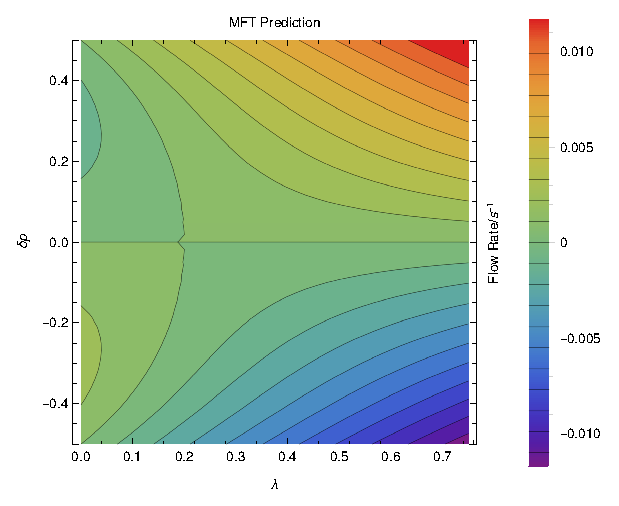
\includegraphics[width=0.5\linewidth]{../tex-src/images/constDens/newMftPred} & 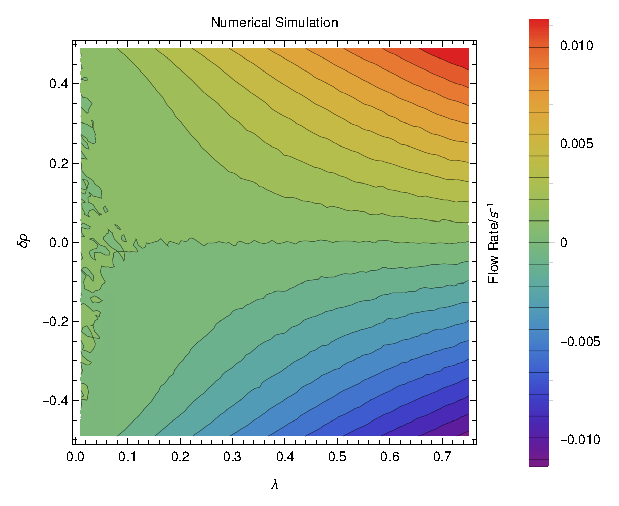
\includegraphics[width=0.5\linewidth]{../tex-src/images/constDens/newFlow} \\
    \hline
    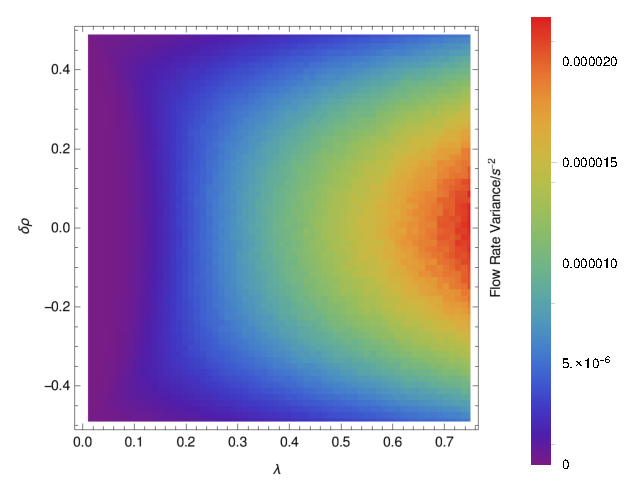
\includegraphics[width=0.5\linewidth]{../tex-src/images/constDens/newVar} & 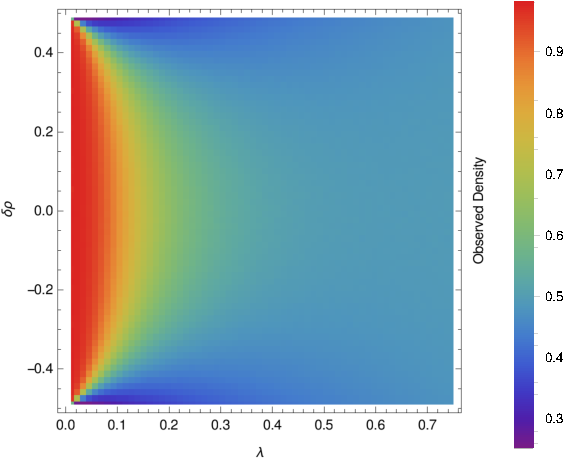
\includegraphics[width=0.5\linewidth]{../tex-src/images/constDens/newDens} \\
    \end{tabular}
\end{center}
    \vspace{-0em}
\end{figure*}
\fi
\begin{figure}[h!]
\vspace{1em}
\caption{\label{fig:constDens} Flow rate mean observed when varying the difference $\delta\rho$ between the boundary concentrations
$(\rho_B, \rho_T) = (\rho_M + \frac{1}{2} \delta\rho, \rho_M - \frac{1}{2} \delta\rho)$ and $\lambda$ (The top panel is the MFT prediction
for the flow rate, whilst bottom shows the observed mean flow rate).
We chose $\rho_M=\frac{1}{2}$, as this gives us the biggest range of $\delta\rho$ to investigate.
These calculations were performed with the same run parameters (system length etc)
as above.}
\begin{center}
 \begin{tabular}{c}
    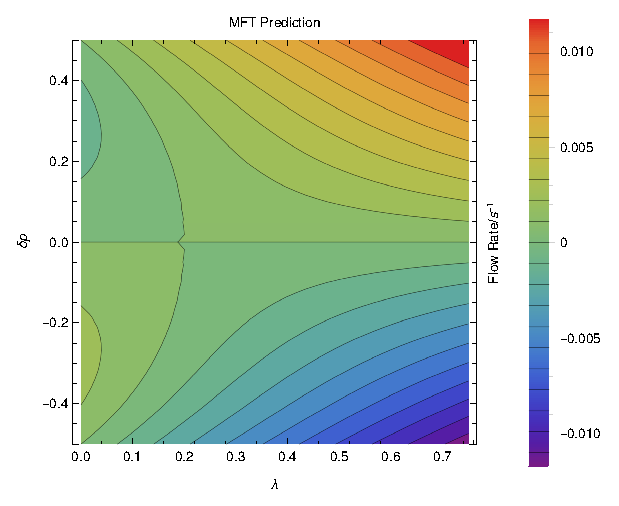
\includegraphics[width=0.98\linewidth]{../tex-src/images/constDens/newMftPred} \\
    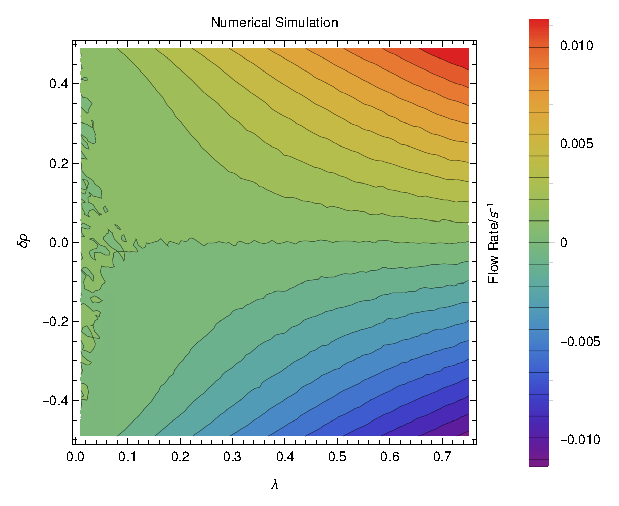
\includegraphics[width=0.98\linewidth]{../tex-src/images/constDens/newFlow}
    \end{tabular}
\end{center}
    \vspace{-2.5em}
\end{figure}
The MFT prediction for the mean flow is generally in good agreement with the numerics, except in the very sticky regime in which flow is very small.
The simulations show no evidence of negative diffusion; rather the flow becomes critically slow for very sticky particles.
The higher moments of the flow (e.g. variance) do not show peaks, indicating that hard transitions are not occurring.
Finally, the density is very close to the average of the boundary densities until λ drops below 1/4, at which point the stickiness causes the system to fill.

Continuing to specify the boundary densities to be $(\rho_0, \rho_L) = (\rho_M + \frac{1}{2} \delta\rho, \rho_M - \frac{1}{2} \delta\rho)$ for some given $\rho_M$, we can keep $\delta\rho$ relatively small, so that $J$ varies approximately
linearly with $\delta\rho$; thus if we calculate $J$ for a series of small $\delta \rho$, we can perform linear regression to find $D_\mathrm{Eff}=\partDeriv{J}{\delta\rho}\big|_{\delta\rho=0}$, the effective diffusion coefficient.
Computing this for different $(\rho_M, \lambda)$ combinations yields results that can be compared with Eq.~\ref{eq:MFTflow}.
\begin{figure}[h!]
\vspace{1em}
\caption{\label{fig:diffCoef}
Comparison of effective diffusion coefficient $D$ in the MFT (top) and in direct simulation (bottom) as a function of density and stickiness.
The white region is where the MFT gives negative diffusion. The simulations used 124 sites averaged over $\sim 10^9$ steps at each of $12 \times 24 \times 16 $ $(\lambda, \rho_M, \delta \rho)$ combinations.
Full details in the supplementary materials.
\iffalse
The top contour plot shows the MFT prediction of the effective diffusion coefficient $D=\partDeriv{J}{\delta\rho}\big|_{\delta\rho=0}$ as a function of local density $\rho_M$ and $\lambda$;
we are only plotting where $0 \le D \le 1.2$, other regions are shown in white, including the region in which $D<0$, which would cause instabilities and so prevent a flow from actually occurring.
Bottom is our numerical calculation of $D(\rho_M, \lambda)$,
with exactly the same plotting ranges.
In this setup we ran the simulation for
$1.6\times10^8$ equilibration steps, followed by $10$ sets of alternating measurement and relaxation runs, of lengths $8\times10^7$ and $1.6\times10^7$ steps respectively. These results are consistent with calculations performed on smaller
systems, so we should be safe from finite-size effects.
\fi
}
\iffalse
\begin{center}[h!]
 \begin{tabular}{c@{\hspace{1em}}c}
    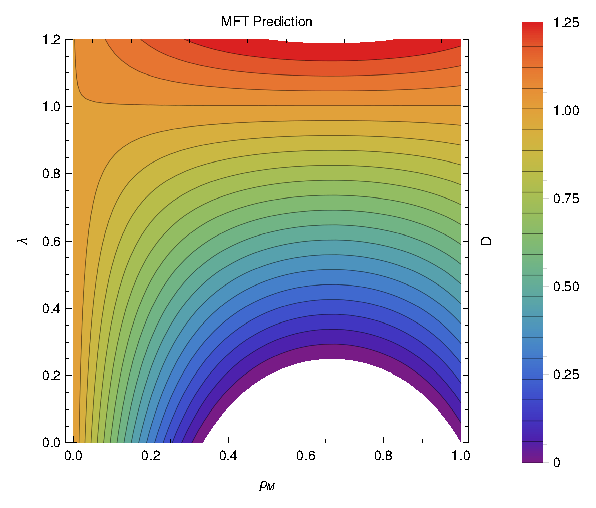
\includegraphics[width=0.5\linewidth]{../tex-src/images/newAnalFlow} & 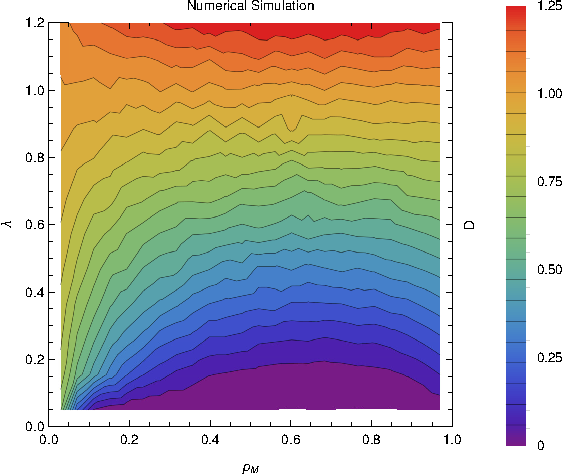
\includegraphics[width=0.5\linewidth]{../tex-src/images/newDataFlow} \\
    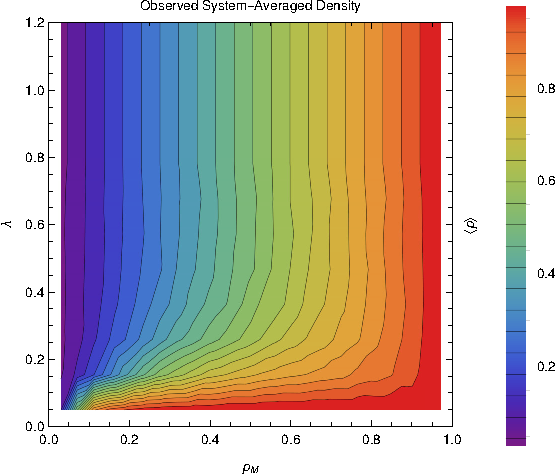
\includegraphics[width=0.5\linewidth]{../tex-src/images/newFlowDens} & 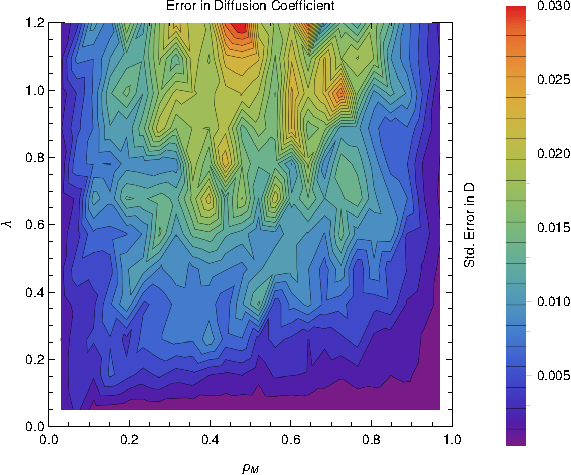
\includegraphics[width=0.5\linewidth]{../tex-src/images/newFlowErr} 
    \end{tabular}
\end{center}
    \vspace{-3em}
\end{figure*}
\fi
%REMEMBER TO ACTUALLY PUT IT THERE!!!
\begin{center}
 \begin{tabular}{c}
    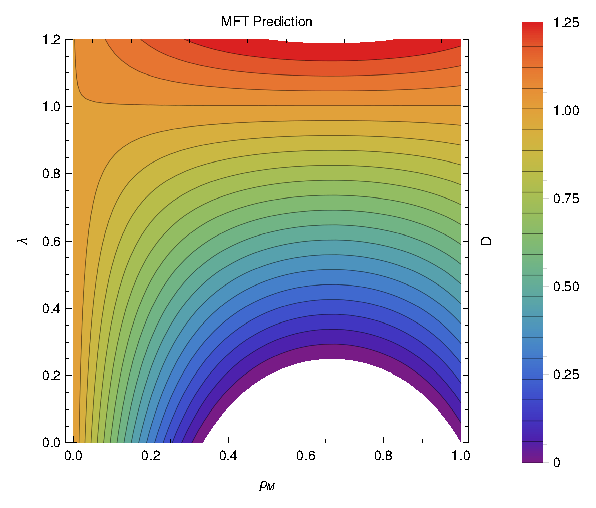
\includegraphics[width=0.98\linewidth]{../tex-src/images/newAnalFlow} \\
    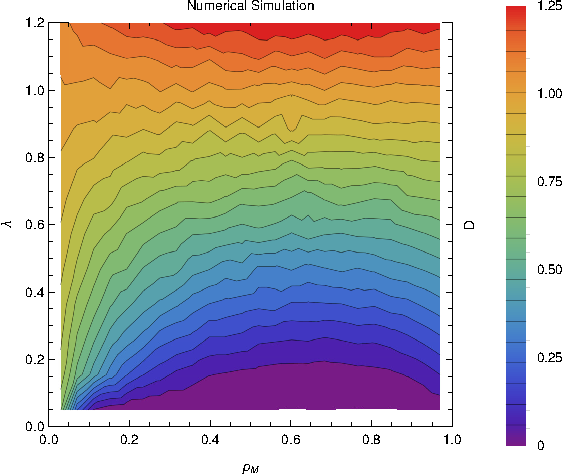
\includegraphics[width=0.98\linewidth]{../tex-src/images/newDataFlow}
    \end{tabular}
\end{center}
    \vspace{-2em}
\end{figure}

One can compare the MFT prediction and the actual numerical results together as we have done in Fig.~\ref{fig:diffCoef}. We see that MFT and simulation agree well for low stickiness, and both show the symmetry
about $\rho_M = \frac{2}{3}$. For high stickiness, where the MFT prediction gives negative diffusion constant, the simulation generates a much increased density in the system.  This takes $\rho_M$ outside the negative-$D$ regime of the MFT,
and into slow, but positive $D$ regime; this might explain why our measured diffusion coefficients seem to have been ``stretched'' along the $\rho_M$ axis. As before, we don't see a consistent spiking in the variance of the flow rate,
which is generally consistent with out other findings with
regards to the accuracy of the MFT.
%Query

%The structure of the flow is shown in Fig 5.  We observe density correlations persisting over many sites and for very long timescales.  These high and low density structures show no systematic movement.
%Superimposed on the pattern we see narrow lines with well defined gradient (velocity) which we believe correspond to individual particles/vacancies diffusing through regions of low/high density.
It is instructive to get an overview of how the particles move during flow. Fig.~\ref{fig:flowPatterns} show a plot of the flow structure in an interesting regime.
We note that over short timescales little structure is visible, the dynamics appearing as a random walk with some tendency for particles to clump; over longer timescales the diffusive behavior is more evident, with a textured structure suggesting characteristic velocity of  particles or vacancies through emergent correlated clumps.
Additional plots can be found in the supplementary materials at [URL will be inserted by publisher].

\begin{figure}[h!]
\caption{\label{fig:flowPatterns} Indicative spacetime flow pattern for sticky free-flow $\left[\lambda = \frac{3}{20}, (\rho_0, \rho_L) = (\frac{3}{4}, \frac{1}{4})\right]$; other combinations shown in the supplementary materials.
Time runs along the x-axis, space (1 pixel=1 site) along the y-axis, with grayscale tone (black being empty, white being full) illustrating average site occupation over (clockwise from top left) $\frac{1}{32}$, $1$, $8$ and $32$ Gillespie steps per site respectively.}
%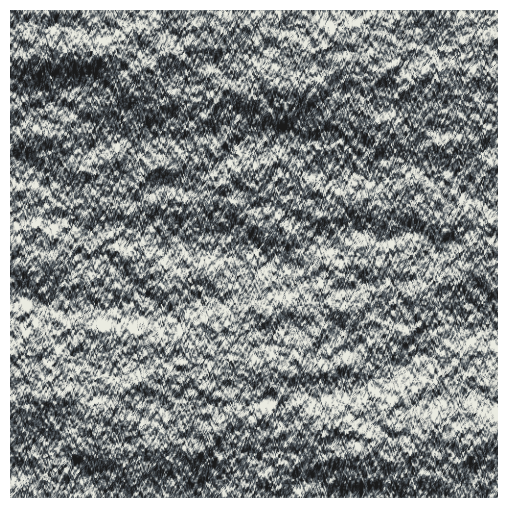
\includegraphics[width=0.98\linewidth]{../tex-src/images/flowImps2/flowl2r2.png}
\begin{center}
 \begin{tabular}{c | c}
    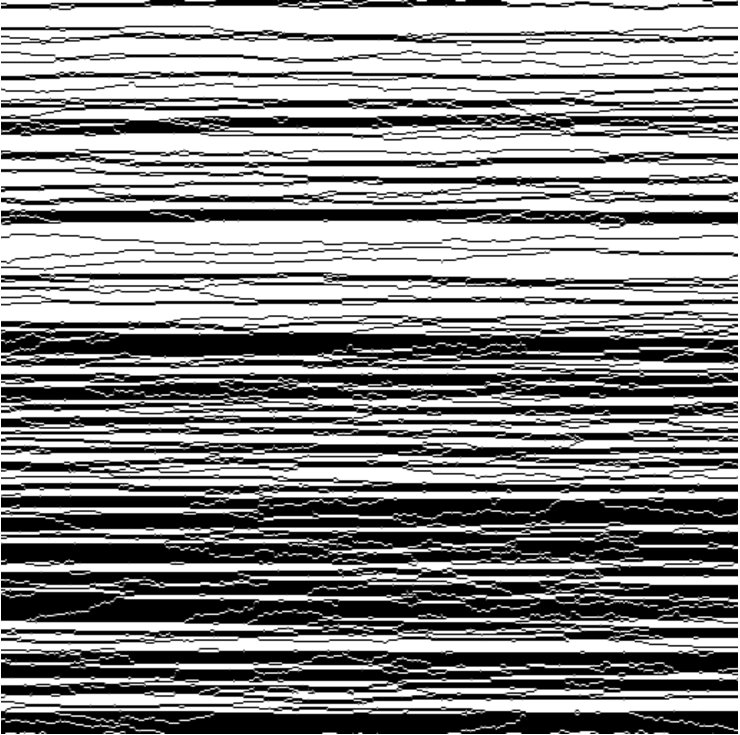
\includegraphics[width=0.49\linewidth]{../tex-src/images/newFlowImps/shortTime}  &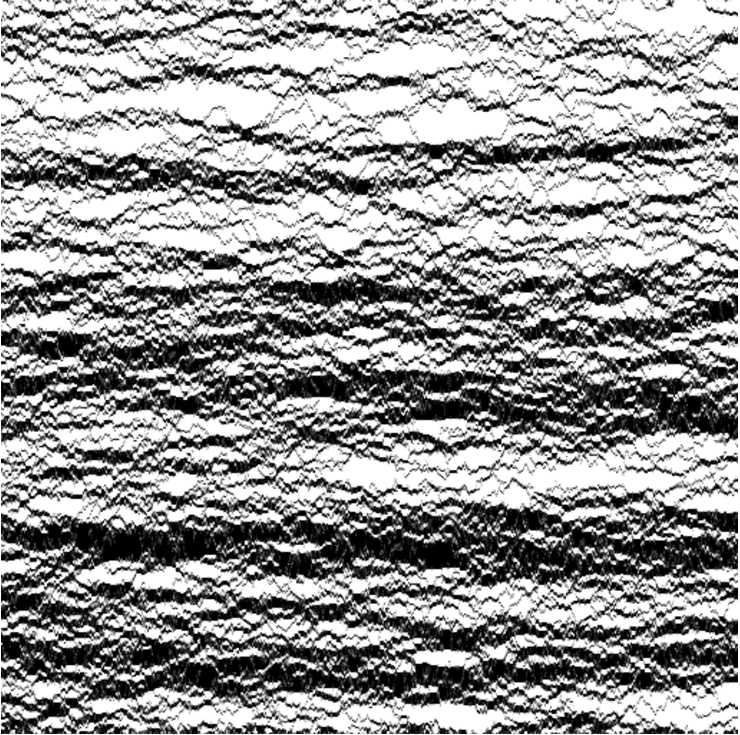
\includegraphics[width=0.49\linewidth]{../tex-src/images/newFlowImps/midShortTime} \\
    \hline
    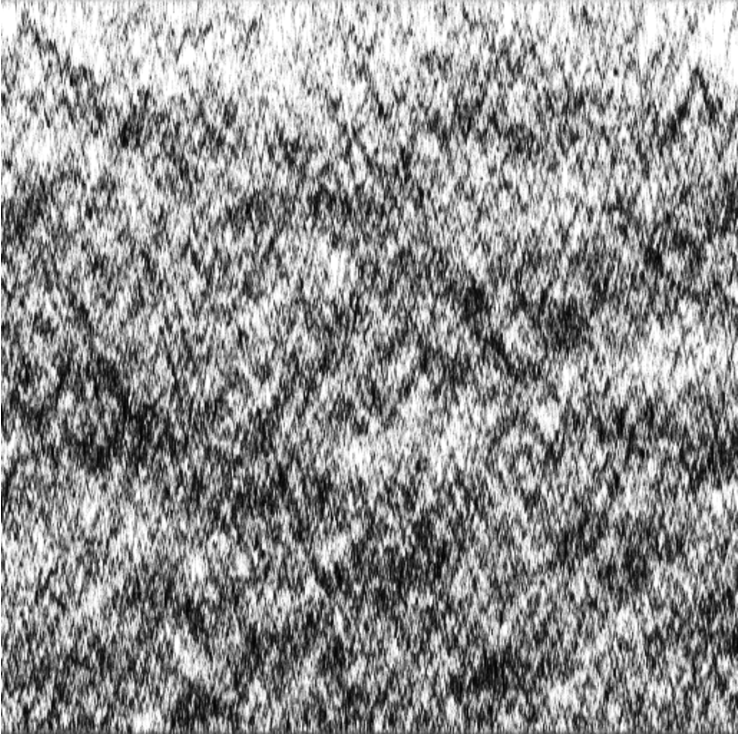
\includegraphics[width=0.49\linewidth]{../tex-src/images/newFlowImps/longTime} &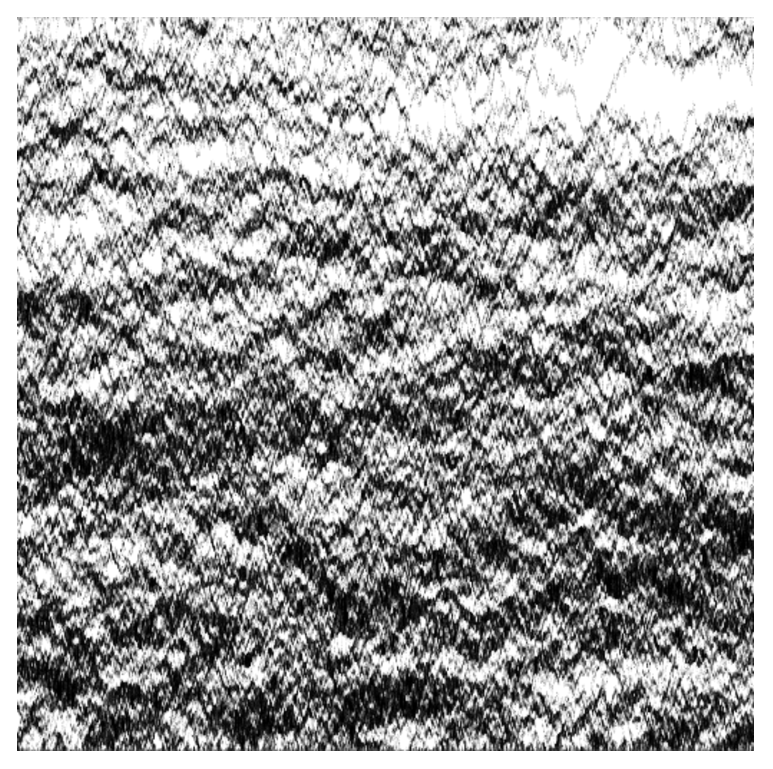
\includegraphics[width=0.49\linewidth]{../tex-src/images/newFlowImps/midLongTime}
    \end{tabular}
\end{center}
    \vspace{-2em}
\end{figure}

\iffalse
Fig.~\ref{fig:flowPatterns} shows the short-time-averaged local density as a function of space and time for a range of densities and stickiness.
\begin{figure*}[h!]
\caption{\label{fig:flowPatterns} The spacetime flow patterns, for the $(\lambda, \rho_M)$ combinations indicated in the row and column headers. In each plot time runs along the $x$-axis, space along the $y$-axis. White represents full occupation, black empty, and grey shades partial
occupation. The degree of occupation was calculated by taking the \texttt{KMCLib} record of a particular site's occupation (i.e. the Gillespie times at
which the site changed occupation), assigning $0$ and $1$ to particles and vacancies respectively, linearly interpolating this and then integrating over times longer than a single Gillespie step but much shorter than the total time in question.
In each case the total time elapsed is that taken by $10^6$ Gillespie steps, and each short-time-average has been done over the total time divided by $508$ (to produce square diagrams, as there are $508$ active sites
per simulation). Time has been rescaled this way in order to allow fair comparison of radically different $\lambda$-values.}
\begin{tabular}{c p{0.175\linewidth}}
\hspace{-2em}\begin{tabular}{c|c@{\hspace{0.25em}}c@{\hspace{0.25em}}c}
  &  $\lambda=0.05$ & $\lambda=0.38$ & $\lambda=1.00$ \\ 
  \hline
   \begin{tabular}{c} \vspace{-12em} \\ \hspace{-1em}$\rho_M=0.05$\hspace{0em} \\  \\ \end{tabular} & 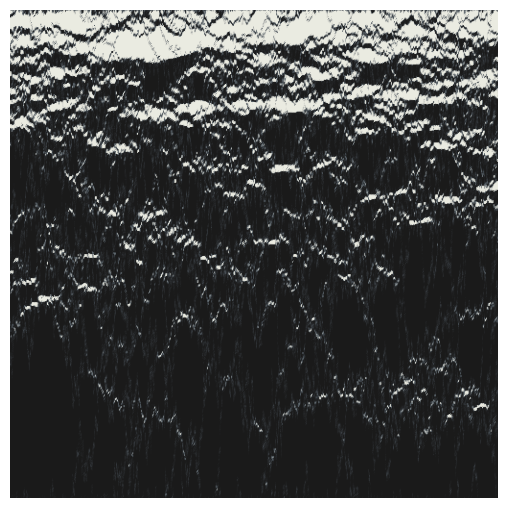
\includegraphics[width=0.32\linewidth]{../tex-src/images/flowImps2/flowl0r0.png} & 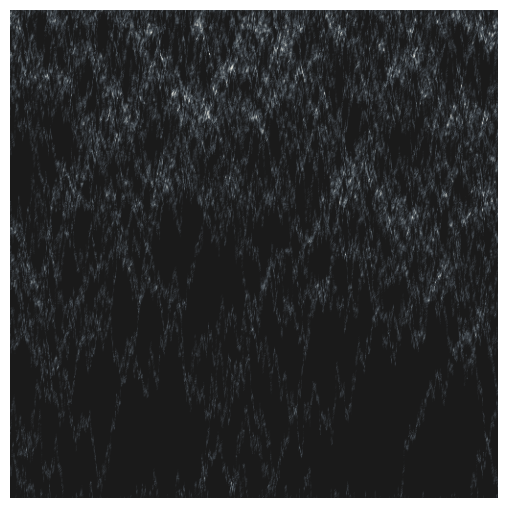
\includegraphics[width=0.32\linewidth]{../tex-src/images/flowImps2/flowl2r0.png}  & 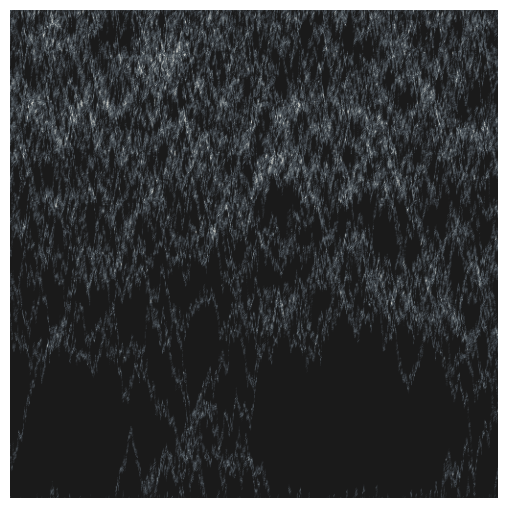
\includegraphics[width=0.32\linewidth]{../tex-src/images/flowImps3/flowl0r0.png} \\
   \begin{tabular}{c} \vspace{-12em} \\ \hspace{-1em}$\rho_M=0.50$\hspace{0em} \\  \\ \end{tabular} & 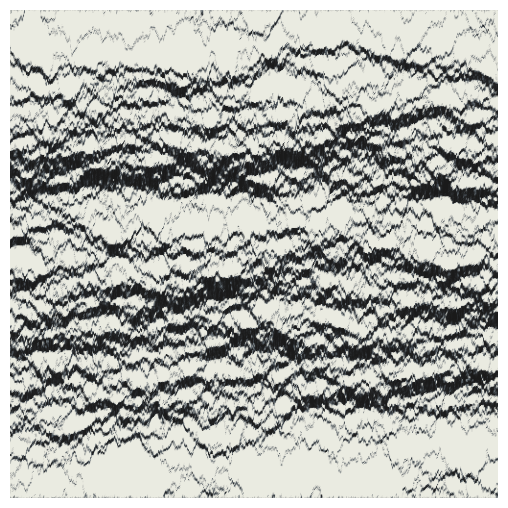
\includegraphics[width=0.32\linewidth]{../tex-src/images/flowImps2/flowl0r2.png} & 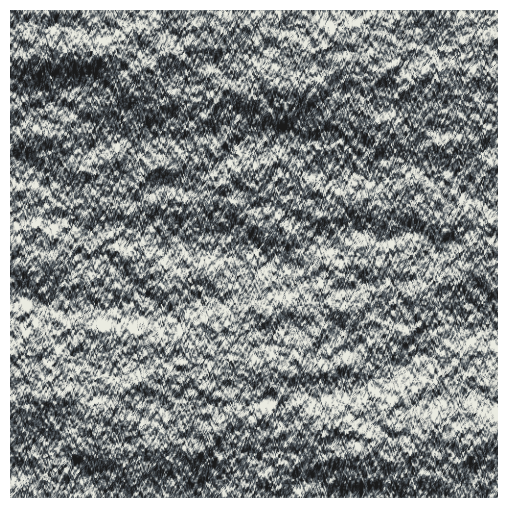
\includegraphics[width=0.32\linewidth]{../tex-src/images/flowImps2/flowl2r2.png}  & 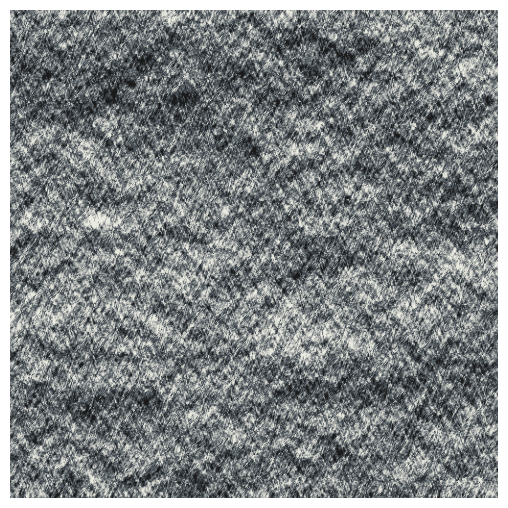
\includegraphics[width=0.32\linewidth]{../tex-src/images/flowImps3/flowl0r2.png} \\
   \begin{tabular}{c} \vspace{-12em} \\ \hspace{-1em}$\rho_M=0.95$\hspace{0em} \\  \\ \end{tabular} & 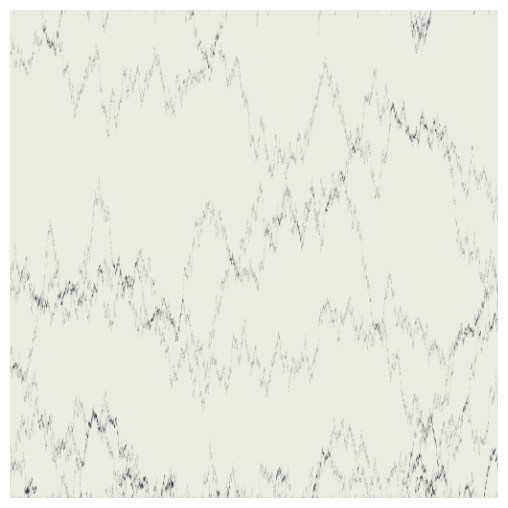
\includegraphics[width=0.32\linewidth]{../tex-src/images/flowImps2/flowl0r4.png} & 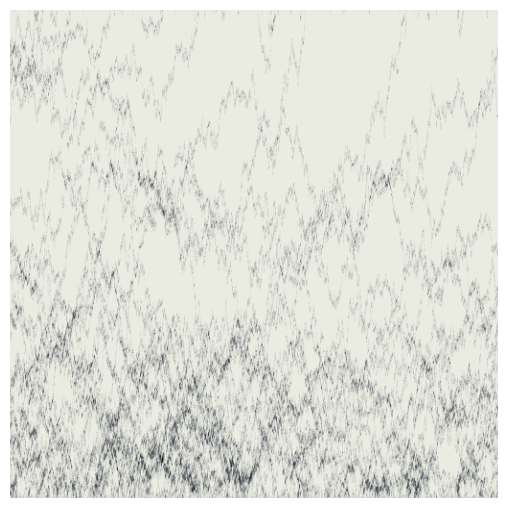
\includegraphics[width=0.32\linewidth]{../tex-src/images/flowImps2/flowl2r4.png}  & 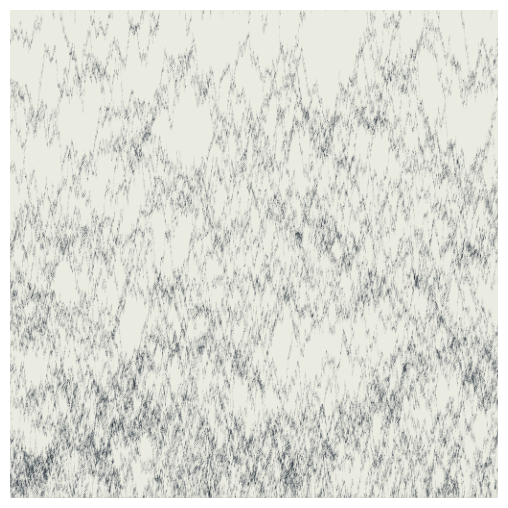
\includegraphics[width=0.32\linewidth]{../tex-src/images/flowImps3/flowl0r4.png} \\
   \end{tabular}
\hspace{-1em}
&
\end{tabular}
\end{figure*}
When $\lambda$ is extremely low (left), the medium consists of solid blocks surrounded by empty spaces containing a dilute
gas of particles; as we alter the overall density, all that changes is the thicknesses of these blocks.   Thus the breakdown of MFT
is revealed as a decomposition into regions, of alternating low and high density, each of which allows similar flow rate.  The MFT solution, which assumed
intermediate density and gave negative diffusion constant, is revealed to be unstable.
The case $\lambda = 1$ (right) is just excluded Brownian motion, and is included here for comparison.
The most interesting images (centre) are those for the intermediate $(\rho_M , \lambda)$; here we see a ``lumpy'' or ``foamy'' structure, in which small blocks
of particles are being constantly created and destroyed whilst a rather minimal flow occurs across the system.
The simulations did not show any hard phase transition as we vary $(\rho_M, \lambda)$; rather, it seems that this ``foamy''
behaviour is part of a continuous range between the extremes, containing medium-range correlations between particles.
Unfortunately, computing equal-time correlation functions to the accuracy required
to draw conclusions about these correlations has proven to be extremely difficult, so we cannot find a quantitative description of the foam beyond the averages properties in Fig.~\ref{fig:lambdaScans}, \ref{fig:constDens},
and \ref{fig:diffCoef}.
In all images in Fig.~\ref{fig:flowPatterns}, long straight segments of white of black can be seen.  The represent coherent motion at a characteristic velocity given by their gradient. There is nothing in the MFT to suggest what this velocity
should be, and it is much smaller than the simulated system's length divided by the elapsed time,  $\frac{L}{T}$, thus it must be an emergent property arising from correlated motion of self-assembled regions of  high- or low-density material.

When $\lambda$ is extremely low, the medium consists of solid blocks surrounded by empty spaces containing a dilute gas of particles; as we alter the overall density,
all that changes is the thicknesses of these blocks. The case $\lambda=1$ is just excluded Brownian motion, and is included here for comparison. The most interesting images are those for the intermediate $(\rho_M , \lambda)$; here
we see a ``lumpy'' or ``foamy'' structure, in which small blocks of particles are being constantly created and destroyed whilst a rather minimal flow occurs across the system.
We do not think that there is any hard phase transition as we vary $(\rho_M , \lambda)$; rather, it seems that this ``foamy'' behaviour is part of a continuous range of phenomena between the extremes, containing medium-range correlations between
particles. However, numerically computing equal-time quantities such as the equal-time correlation function to the accuracy required to draw conclusions about these correlations has proven to be extremely difficult, so we cannot speak in quantitative terms about them.
\fi
\iffalse
\subsection{Correlation Functions}
Whilst we're calculating flow rates, we can also use our \texttt{KMCLib} code to calculate the equal time 2-point correlation function
$C(x) = \left\langle \rho(x)\rho(0) \right\rangle - \left\langle \rho(x) \right\rangle \left\langle \rho(0) \right\rangle $.
We can calculate the same quantity in a finite periodic ring analytically, and in both the analytic and numerical cases we may attempt to extract a correlation length by (curve-fitting / Laplace transform);
hence we can check whether having a steady flow through the system causes any structural effects.}
\fi